\documentclass{article}
\usepackage[a4paper,scale=0.8,hcentering,bindingoffset=8mm]{geometry} % A4纸大小,缩放80%,设置奇数页右边留空多一点
\usepackage{hyperref}      % 超链接
\usepackage{listings}      % 代码块
\usepackage{courier}       % 字体
\usepackage{fontspec}      % 字体
\usepackage{fancyhdr}      % 页眉页脚相关宏包
\usepackage{lastpage}      % 引用最后一页
\usepackage{amsmath,amsthm,amsfonts,amssymb,bm} %数学
\usepackage{graphicx}      % 图片
\usepackage{subcaption}    % 图片描述
\usepackage{longtable,booktabs} % 表格
\usepackage{ctex}
\usepackage{soul}
\usepackage{dot2texi}
\usepackage{tikz}
\usepackage{multirow}
% \setmainfont{Noto Sans Kaithi}
\usetikzlibrary{automata, positioning, arrows}
\lstset{                  %设置代码块
         basicstyle=\footnotesize\ttfamily,% 基本风格
         numbers=left,    % 行号
         numbersep=10pt,  % 行号间隔 
         tabsize=4,       % 缩进
         extendedchars=true, % 扩展符号?
         breaklines=true, % 自动换行
         language=C,
         frame=leftline,  % 框架左边竖线
         xleftmargin=5pt,% 竖线左边间距
         showspaces=false,% 空格字符加下划线
         showstringspaces=false,% 字符串中的空格加下划线
         showtabs=false,  % 字符串中的tab加下划线
 }
\pagestyle{fancy}         % 页眉页脚风格
\fancyhf{}                % 清空当前设置
\fancyfoot[C]{\thepage\ / \pageref{LastPage}}%页脚中间显示 当前页 / 总页数,把\label{LastPage}放在最后
\begin{document} 
    \begin{titlepage}       % 封面
        \centering
        
\includegraphics[width=\textwidth]{../SUSTC_LOGO.png}
        % \vspace*{\baselineskip}
        \rule{\textwidth}{1.6pt}\vspace*{-\baselineskip}\vspace*{2pt}
        \rule{\textwidth}{0.4pt}\\[\baselineskip]
        {\LARGE COMPILIER @Liu Yepang 2019\\[\baselineskip]\small for SUSTech CSE}
        \\[0.2\baselineskip]
        \rule{\textwidth}{0.4pt}\vspace*{-\baselineskip}\vspace{3.2pt}
        \rule{\textwidth}{1.6pt}\\[\baselineskip]
        \scshape
        \vspace*{\baselineskip}
        {\Large HomeWork 3\par }
        Edited by \\[\baselineskip] {汪至圆\par}
        {\Large 11610634\par }
        \vfill
        {\scshape 2019} \\{\large SHENZHEN}\par
    \end{titlepage}
    \section{Consider the following context-free grammar G}
        $$S \rightarrow S S+|S S *| a$$
        \subsection{Is the string a+a∗a in L(G)? [20 points]:}
            No, it isn't in L(G). For this grammar, the first two character of the string
            must be aa or the string just have a single character a.
        \subsection{Give a leftmost derivation for the string aa∗aa+∗. [20 points]:}
            $$S\rightarrow SS*\rightarrow SS*S*\rightarrow aS*S*\rightarrow aa*S*\rightarrow aa*SS+*\rightarrow aa*aS+*\rightarrow aa*aa+*$$
        \subsection{Give a rightmost derivation for the stringaa∗aa+∗. [20 points]:}
            $$S\rightarrow SS*\rightarrow SSS+*\rightarrow SSa+*\rightarrow Saa+*\rightarrow SS*aa+*\rightarrow Sa*aa+*\rightarrow aa*aa+*$$
        \subsection{ Give a parse tree for the string aa ∗ aa + ∗. [20 points]:}
            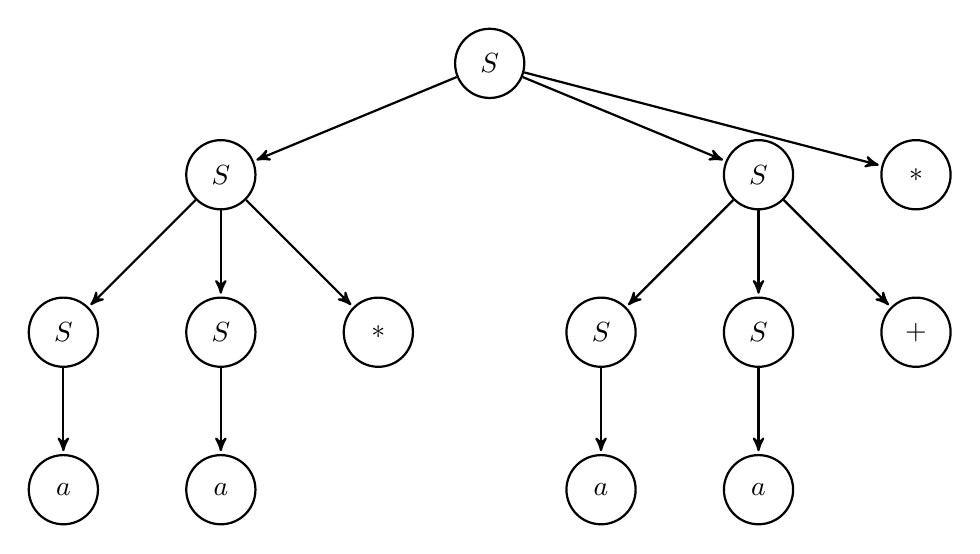
\begin{tikzpicture}[->,>=stealth',shorten >=1pt,auto,node distance=2cm,
                thick,base node/.style={circle,draw,minimum size=16pt}, real node/.style={double,circle,draw,minimum size=35pt}]
                \node[state] (1) {$S$};
                \node(temp1) [below right of = 1]{};
                \node(temp2) [below left of = 1 ]{};
                \node[state] (2) [right of=temp1] {$S$};
                \node[state] (3) [left of=temp2] {$S$};
                \node[state] (4) [right of=2] {$*$};
                \node[state] (5) [below of=3] {$S$};
                \node[state] (6) [left of=5] {$S$};
                \node[state] (7) [right of=5] {$*$};
                \node[state] (8) [below of=2] {$S$};
                \node[state] (9) [left of=8] {$S$};
                \node[state] (10) [right of=8] {$+$};
                \node[state] (11) [below of=5] {$a$};
                \node[state] (12) [below of=6] {$a$};
                \node[state] (13) [below of=8] {$a$};
                \node[state] (14) [below of=9] {$a$};
                \path[]
                (1) edge node {} (2)
                (1) edge node {} (3)
                (1) edge node {} (4)
                (3) edge node {} (5)
                (3) edge node {} (6)
                (3) edge node {} (7)
                (2) edge node {} (8)
                (2) edge node {} (9)
                (2) edge node {} (10)
                (5) edge node {} (11)
                (6) edge node {} (12)
                (8) edge node {} (13)
                (9) edge node {} (14)
                ;
            \end{tikzpicture}
        \subsection{Give an equivalent grammar without immediate left recursions. [20 points]}
            $S\rightarrow aS'$

            $S'\rightarrow S+S'|S*S'|\epsilon$    
    
    \section{Optional Exercises (20 bonus points)}
        \subsection{Exercise 1: Consider the following context-free grammar:}
            $$\text{短语}\rightarrow \text{人|短语}\quad\text{动词}\quad\text{短语}$$
            $$\text{动词} \rightarrow \text{喜欢 | 不喜欢} $$
            $$\text{人}\rightarrow \text{你 | 我 | 他}$$
            The grammar can produce sentences such as “我喜欢你”. Is the grammar ambiguous? If yes,
            please give one sentence and its multiple parse trees. If no, state the reason. [5 points for
            the yes/no answer and 15 points for the justification]
            
            Yes, it's ambiguous.
            For example, for the sentence "我不喜欢他喜欢你", we can get two parse tree like below:

            \begin{tikzpicture}[->,>=stealth',shorten >=1pt,auto,node distance=2.5cm,
                thick,base node/.style={circle,draw,minimum size=2cm}, real node/.style={double,circle,draw,minimum size=35pt}]
                \node[state] (1) {短语};
                \node(temp1) [below right of = 1]{};
                \node(temp2) [below left of = 1 ]{};
                \node[state] (2) [right of=temp1] {动词};
                \node[state] (3) [left of=temp2] {短语};
                \node[state] (4) [right of=2] {短语};
                \node[state] (5) [below of=3] {动词};
                \node[state] (6) [left of=5] {短语};
                \node[state] (7) [right of=5] {短语};
                \node[state] (8) [below of=2] {喜欢};
                \node[state] (9) [below of=4] {人};
                \node[state] (10) [below of=5] {不喜欢};
                \node[state] (11) [below of=6] {人};
                \node[state] (12) [below of=7] {人};
                \node[state] (13) [below of=11] {我};
                \node[state] (14) [below of=12] {他};
                \node[state] (15) [below of=9] {你};
                \path[]
                (1) edge node {} (2)
                (1) edge node {} (3)
                (1) edge node {} (4)
                (3) edge node {} (5)
                (3) edge node {} (6)
                (3) edge node {} (7)
                (2) edge node {} (8)
                (4) edge node {} (9)
                (6) edge node {} (11)
                (7) edge node {} (12)
                (5) edge node {} (10)
                (11) edge node {} (13)
                (12) edge node {} (14)
                (9) edge node {} (15)
                ;
            \end{tikzpicture}

            \begin{tikzpicture}[->,>=stealth',shorten >=1pt,auto,node distance=2.5cm,
                thick,base node/.style={circle,draw,minimum size=2cm}, real node/.style={double,circle,draw,minimum size=35pt}]
                \node[state] (1) {短语};
                \node(temp1) [below right of = 1]{};
                \node(temp2) [below left of = 1 ]{};
                \node[state] (2) [left of=temp2] {动词};
                \node[state] (3) [right of=temp1] {短语};
                \node[state] (4) [left of=2] {短语};
                \node[state] (5) [below of=3] {动词};
                \node[state] (6) [left of=5] {短语};
                \node[state] (7) [right of=5] {短语};
                \node[state] (8) [below of=2] {不喜欢};
                \node[state] (9) [below of=4] {人};
                \node[state] (10) [below of=5] {喜欢};
                \node[state] (11) [below of=6] {人};
                \node[state] (12) [below of=7] {人};
                \node[state] (13) [below of=11] {他};
                \node[state] (14) [below of=12] {你};
                \node[state] (15) [below of=9] {我};
                \path[]
                (1) edge node {} (2)
                (1) edge node {} (3)
                (1) edge node {} (4)
                (3) edge node {} (5)
                (3) edge node {} (6)
                (3) edge node {} (7)
                (2) edge node {} (8)
                (4) edge node {} (9)
                (6) edge node {} (11)
                (7) edge node {} (12)
                (5) edge node {} (10)
                (11) edge node {} (13)
                (12) edge node {} (14)
                (9) edge node {} (15)
                ;
            \end{tikzpicture}
            
\end{document}